\documentclass[12pt]{article}
\usepackage[margin=0.75in]{geometry}
\geometry{a4paper}
\usepackage[T1]{fontenc} % Support Icelandic Characters
\usepackage[utf8]{inputenc} % Support Icelandic Characters
\usepackage{graphicx} % Support for including images
\usepackage{hyperref} % Support for hyperlinks
\usepackage{listings}
%------------------------------------------------------------------
% Titill
%------------------------------------------------------------------
\title{
    \vspace{0.5 cm}
    Credit Card Fraud Detection Project Report
}


%------------------------------------------------------------------
% Skjal byrjar hér
%------------------------------------------------------------------
\begin{document}
\maketitle 

\section{Introduction}

This project focuses on developing a model to detect credit card fraud using a highly imbalanced dataset from Kaggle, which includes 284,807 credit card transactions with only 492 identified as fraudulent. The extreme imbalance,\textbf{ where fraudulent transactions make up only 0.17\% of the total}, poses a significant challenge for traditional machine learning techniques.

\hfill \break
To address the class imbalance and improve the detection of fraudulent transactions, \textbf{this project implements three approaches: a voting classifier, a neural network with focal loss, and a synthetic minority oversampling technique (SMOTE).}

\section{Data Analysis}

It \textbf{contains only numerical input variables} which are the result of a PCA transformation. Features V1, V2, … V28 are the principal components obtained with PCA, the only features which have not been transformed with PCA are 'Time' and 'Amount'. Feature 'Time' contains the seconds elapsed between each transaction and the first transaction in the dataset. The feature 'Amount' is the transaction Amount. Feature 'Class' is the response variable and it takes value 1 in case of fraud and 0 otherwise.

\begin{figure}
    \centering
    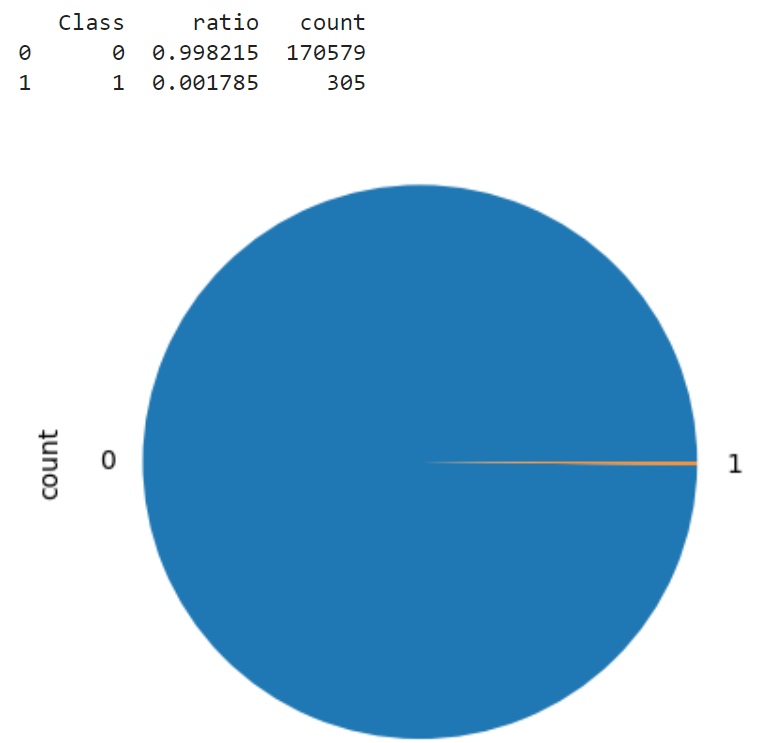
\includegraphics[width=0.40\linewidth]{class_Ratio.png}
    \caption{check class imbalance}
    \label{fig: Check class imbalance}
\end{figure}

\section{Data Correlation}

As you can see in Figure \ref{fig:Correlation Matrix}, There are different correlations or patterns between the feature and each class.    

\hfill \break
\noindent\textbf{Fraud Transactions (Left Heatmap)}

\textbf{Strong Correlations:}
\begin{itemize}
    \item There are noticeable blocks of strong positive correlations among several variables.
    \item Variables such as V1, V2, V3, V4, V5, V6, V7, V8, V9, V10, V11, and V12 show significant correlations among themselves. This is evident from the bright yellow blocks in these regions.
    \item Variables like V16, V17, and V18 also show strong correlations with each other.
\end{itemize}

\bigskip

\noindent\textbf{Non-Fraud Transactions (Right Heatmap)}

\textbf{Weak Correlations:}
\begin{itemize}
    \item The non-fraud transactions heatmap shows mostly weak correlations among variables. The majority of the correlations are close to zero, indicated by the dominance of green and blue colors.
\end{itemize}
\begin{figure}[h]
    \centering
    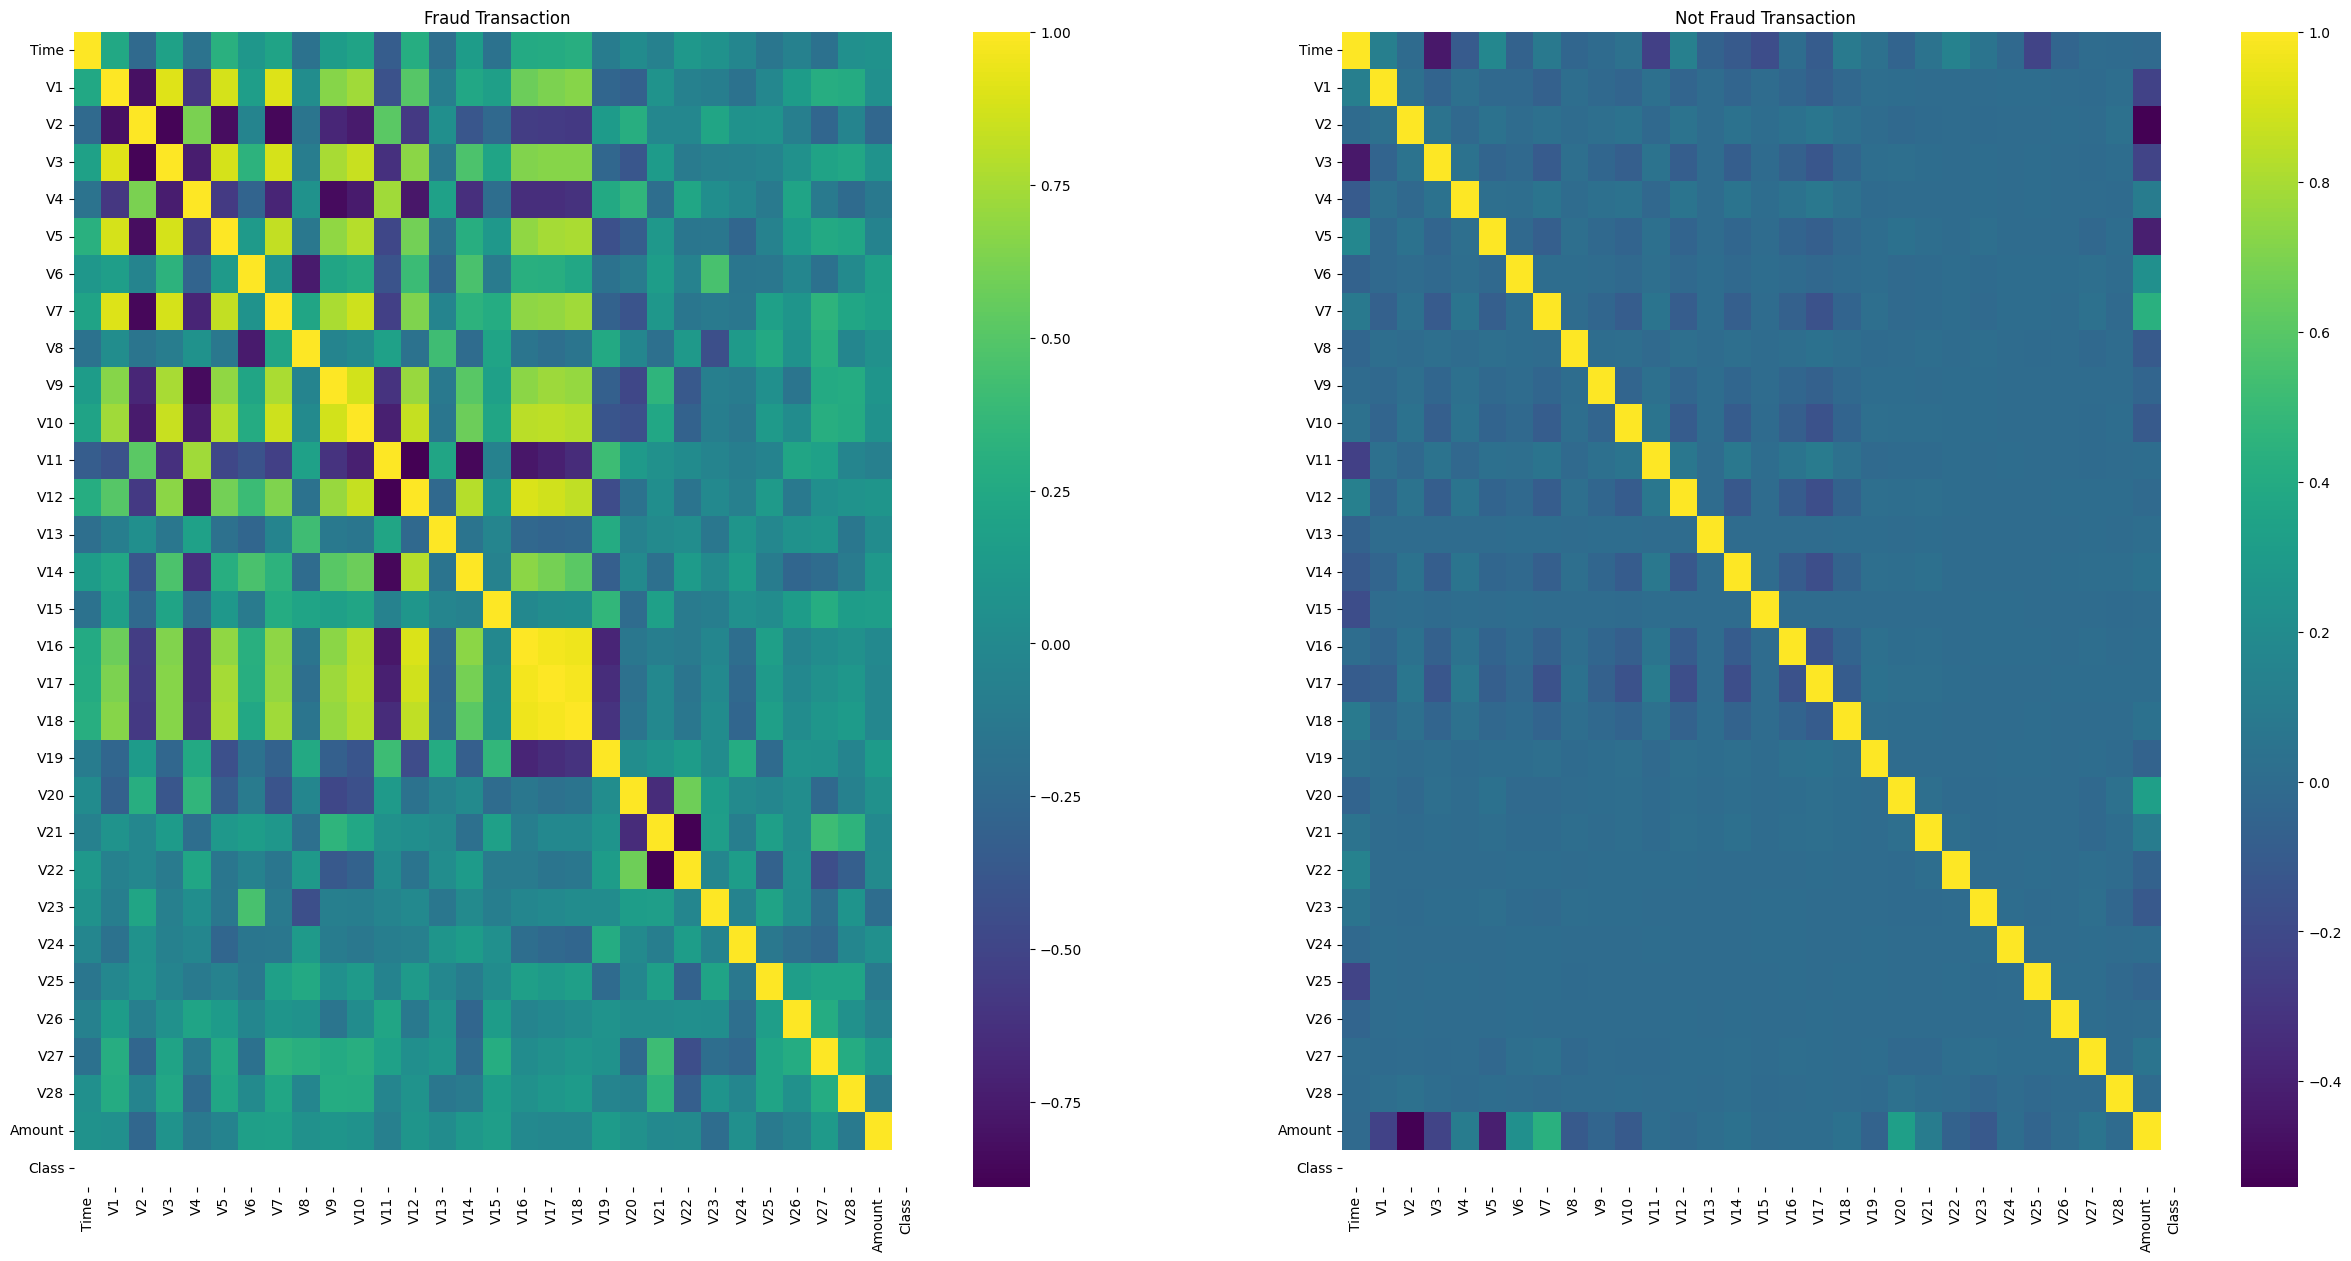
\includegraphics[width=\linewidth]{Correlation Matrix (class separate).png}
    \caption{Correlation matrix separate class}
    \label{fig:Correlation Matrix}
\end{figure}

\newpage

\section{Data visualization using PCA}

As we can see from Figure~\ref{fig:PCA_2D} and Figure~\ref{fig:PCA_3D}, the dataset is highly imbalanced, with Class 0 dominating. There's no clear separation between most of the data points and a few outliers. \textbf{However, we cannot conclude any definitive information because this is just a projection in low dimension.}




\begin{figure}[h]
    \centering
    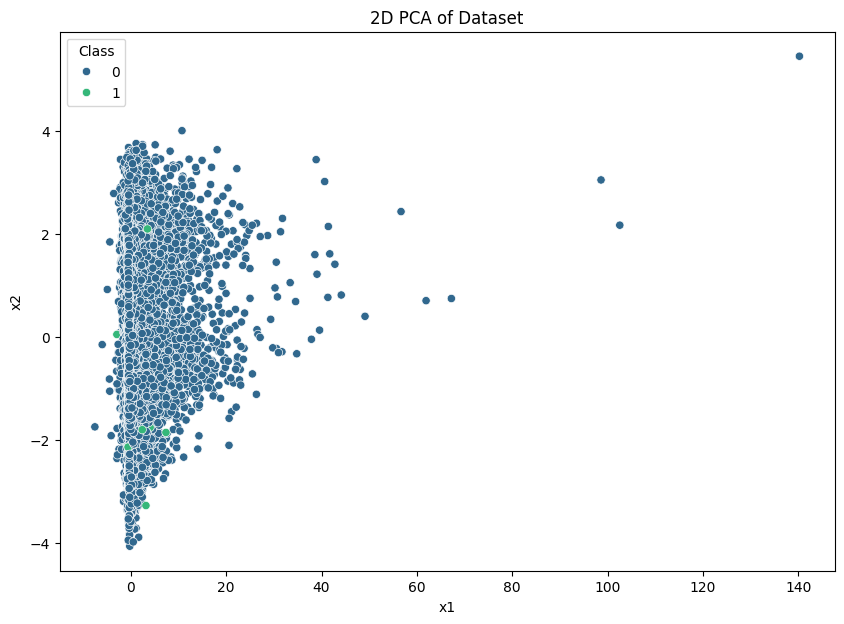
\includegraphics[width=0.5\linewidth]{PCA_2D.png}
    \caption{2D PCA of Dataset}
    \label{fig:PCA_2D}
\end{figure}


\begin{figure}[h]
    \centering
    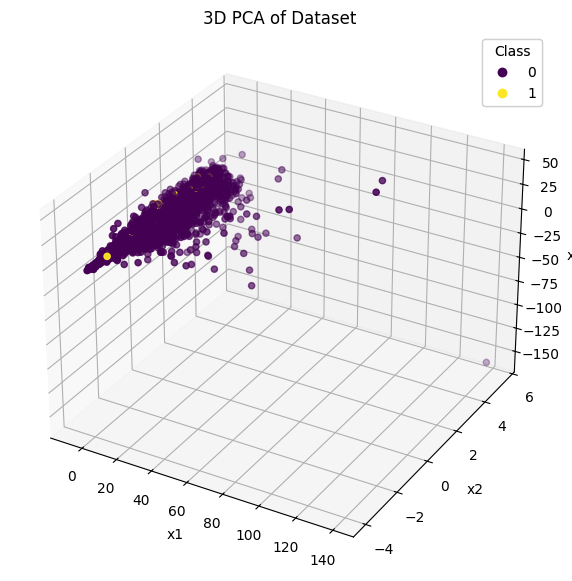
\includegraphics[width=0.5\linewidth]{3D PCA of Dataset.png}
    \caption{3D PCA of Dataset}
    \label{fig:PCA_3D}
\end{figure}
\newpage
\section{Analysis of Random Forest Feature Importances}

The feature importance plot from our Random Forest model provides valuable insights into which features are most influential in predicting credit card fraud. Here's a detailed analysis:

\subsection{Most Important Features}
\begin{itemize}
    \item V17 is by far the most important feature, with a relative importance of approximately 0.2 (20\%).
    \item V14 is the second most important, with importance around 0.17 (17\%).
    \item V12 is third, with importance close to 0.14 (14\%).
\end{itemize}

\subsection{Least Important Features}
Many features (V21, V1, V5, V6, V2, V19, V26, Amount, V13, V8, Time, V15, V20, V25, V22, V28, V24, V23, V27) have very low importance, barely visible on the chart.

\subsection{Key Observations}
\begin{itemize}
    \item The 'Amount' feature has surprisingly low importance, suggesting that the transaction amount alone is not a strong predictor of fraud in this model.
    \item 'Time' also has very low importance, indicating that the time of transaction may not be a crucial factor in detecting fraud.
    \item The features are named V1, V2, etc., which suggests they might be derived features or principal components, possibly from a dimensionality reduction technique applied before the Random Forest model.
\end{itemize}

\begin{figure}[h]
    \centering
    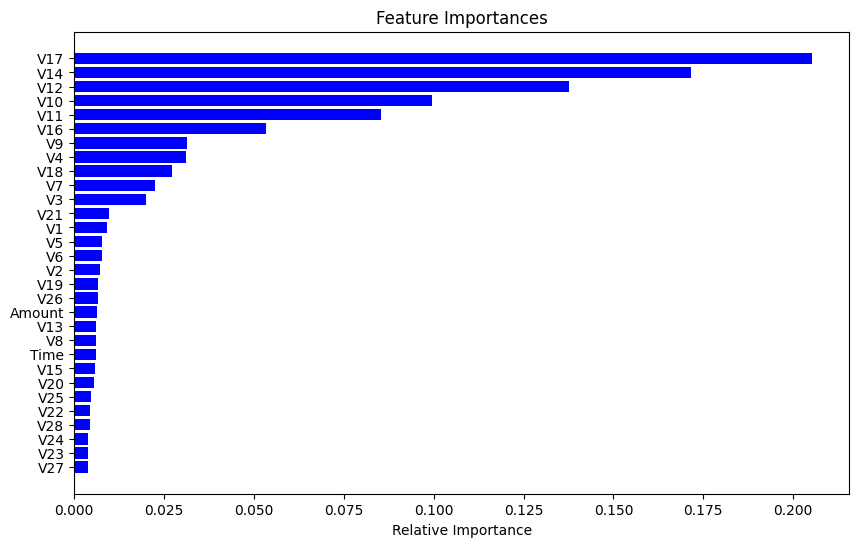
\includegraphics[width=0.8\linewidth]{Random Forest Feature Importances.png}
    \caption{Random Forest Feature Importances}
    \label{fig:Random Forest Feature Importances}
\end{figure}

\newpage
\section{Modeling}
\subsection{Voting Classifier}

I built a voting classifier using three different models: Random Forest, Logistic Regression, and Neural Network.

\paragraph{Random Forest}
I performed a Randomized Search with Stratified K-Fold cross-validation. Additionally, I tried an Extra Trees Classifier. Key observations include:
\begin{itemize}
    \item Random Forests easily overfit the training data.
    \item Regularization techniques very important here.
    \item Increasing the minimum number of samples per leaf helped prevent overfitting.
    \item Normal Random forest outperforms then Extra Trees Classifier.
\end{itemize}

\paragraph{Logistic Regression and KNN}
These classifiers initially achieved poor performance. Notable improvements came from:
\begin{itemize}
    \item Using RobustScaler, which helped more than other scaling techniques.
    \item Setting the \texttt{class\_weight} parameter, which was crucial for performance.
\end{itemize}

\paragraph{Multi-Layer Perceptrons (MLP) - Neural networks}
The MLP achieved the most balance between training and validation performance. Key points from the randomized search with Stratified K-Fold:
\begin{itemize}
    \item Stochastic Gradient Descent (SGD) optimizer performed better than Adam.
    \item The \texttt{tanh} activation function worked better than ReLU.
\end{itemize}


\subsection{Results}
\begin{figure}[h]
    \centering
    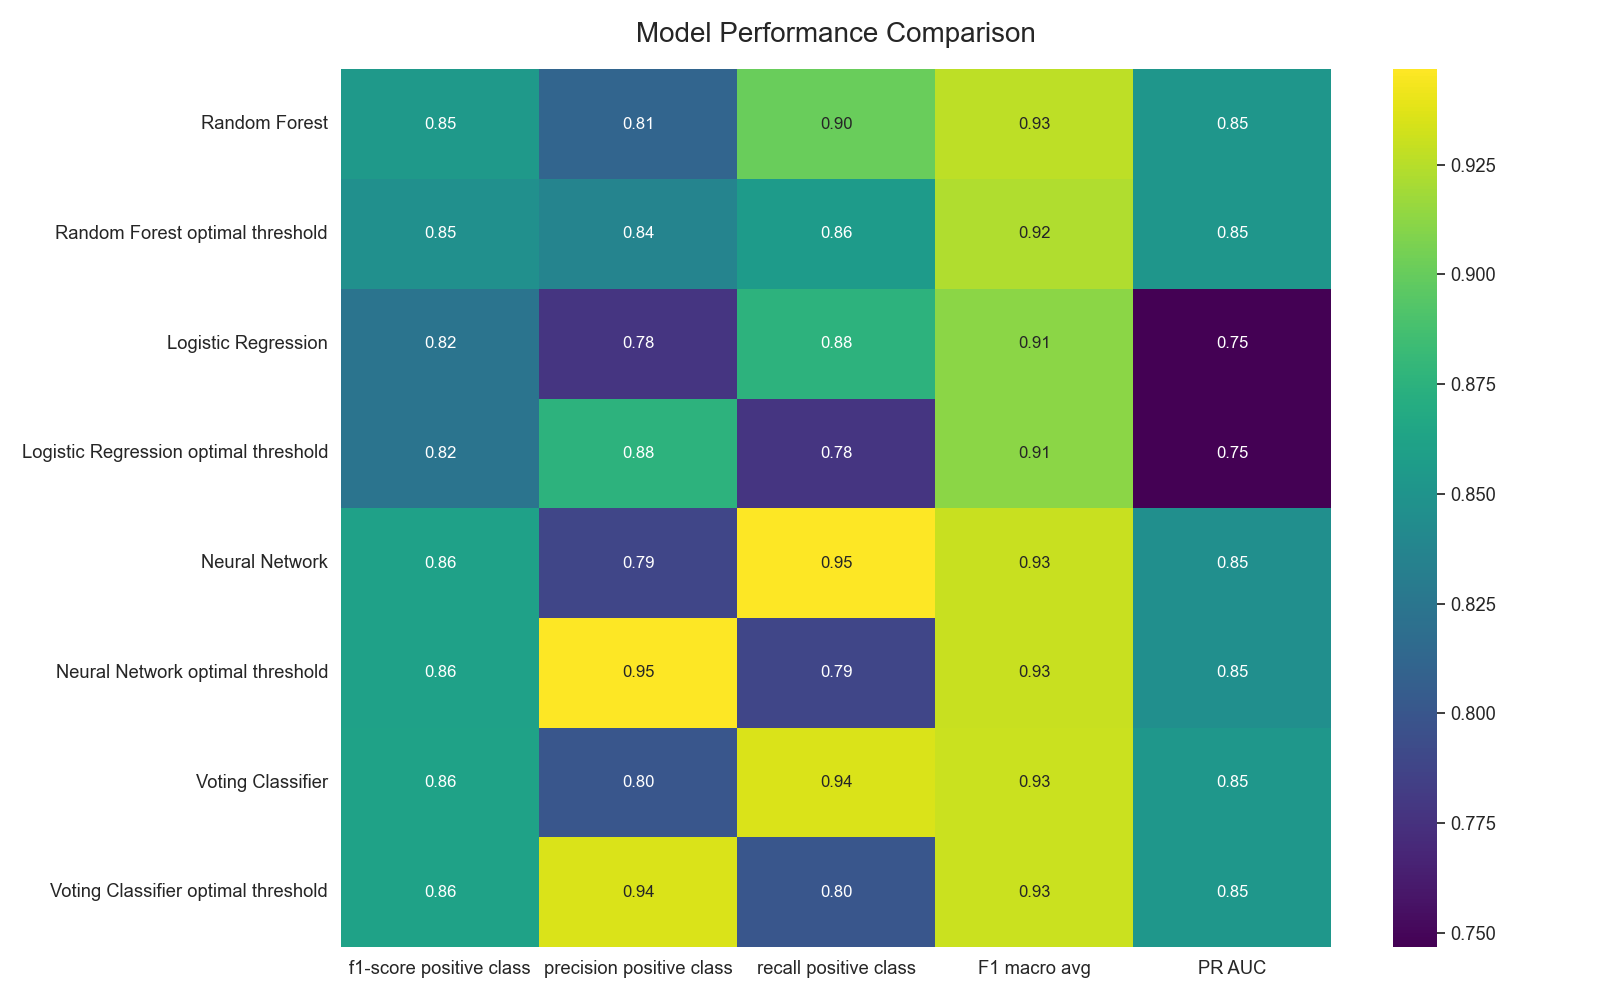
\includegraphics[width=0.74\linewidth]{approach one reaults.png}
    \caption{Model comparison on validation data}
    \label{fig: Model comparison on validation data}
\end{figure}


\newpage
\noindent\textbf{Note:}
\hfill \break
The optimal threshold is calculated by finding the highest F1-score and its threshold in training data only.

\begin{figure}[h]
    \centering
    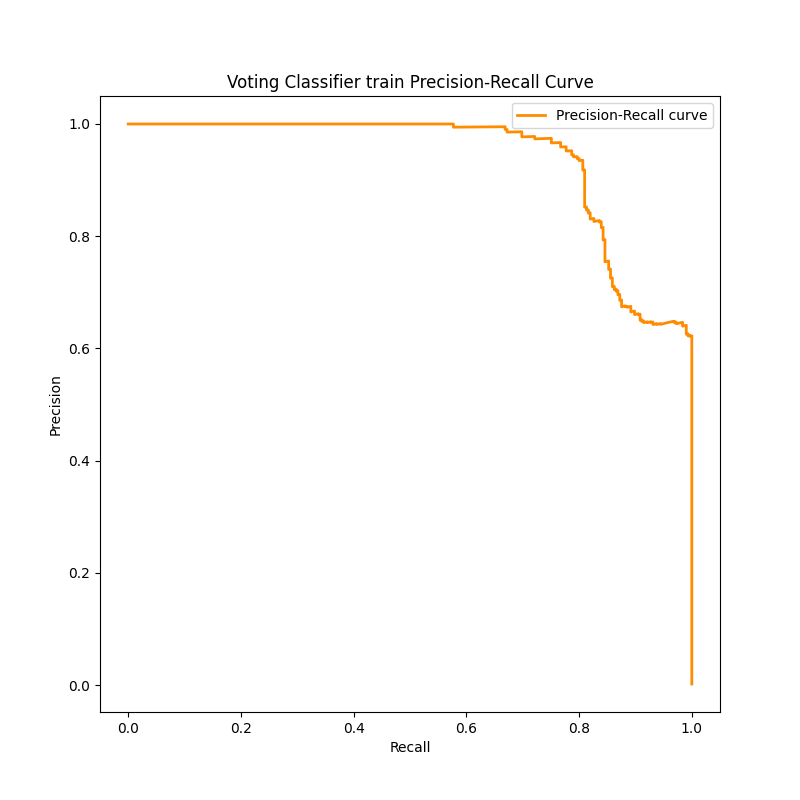
\includegraphics[width=0.5\linewidth]{Voting Classifier train precision recall area under curve.png}
    \caption{Voting Classifier PR-AUC}
    \label{fig:Voting Classifier PR-AUC}
\end{figure}

\begin{figure}[h]
    \centering
    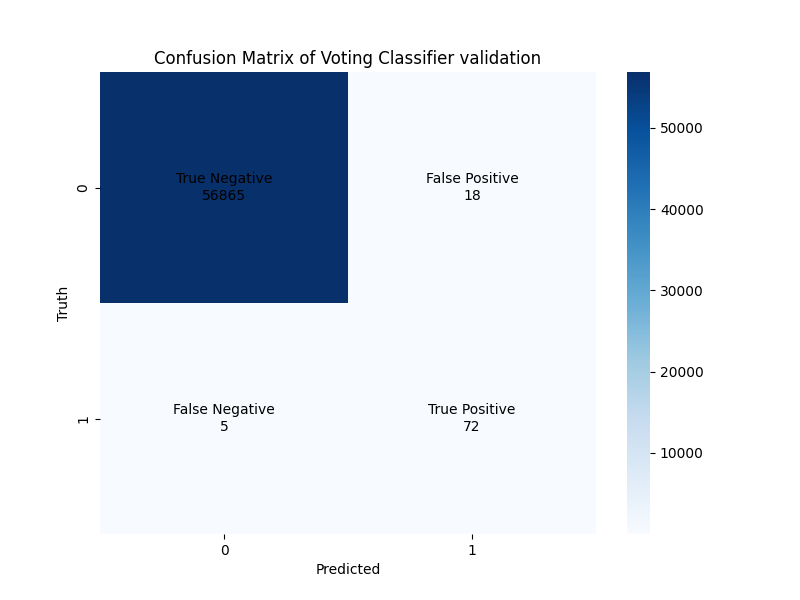
\includegraphics[width=0.65\linewidth]{Voting Classifier validation confusion matrix.png}
    \caption{Voting classifier validation confusion matrix}
    \label{fig:Voting classifier validation confusion matrix}
\end{figure}

\noindent\textbf{Observation:}
\hfill \break
I also observed using K-Nearest Neighbors (KNN) with the \texttt{ball\_tree} algorithm achieved a performance close to that of Random Forest and the neural network but required significantly high computational power.


\newpage
\subsection{Neural network with focal loss}
Focal Loss is a specialized loss function designed to address the class imbalance problem commonly encountered in tasks like object detection. It was introduced in the paper "Focal Loss for Dense Object Detection." The main idea is to focus more on hard-to-classify examples while reducing the loss contribution from easy-to-classify examples. This is achieved through two parameters $\alpha$ (alpha) and $\gamma$ (gamma).

\begin{figure}[h]
    \centering
    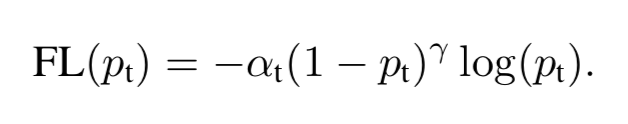
\includegraphics[width=1\linewidth]{Focal_Loss.png}
    \caption{Focal Loss formula}
    \label{fig:Focal Loss formula}
\end{figure}


\begin{lstlisting}[language=Python, caption=My Focal Loss Implementation in PyTorch]
class FocalLoss(nn.Module):
    def __init__(self, gamma=2, alpha=0.25):
        super(FocalLoss, self).__init__()
        self.gamma = gamma
        self.alpha = alpha

    def forward(self, pred_logits, target):
        BCELoss = F.binary_cross_entropy_with_logits(pred_logits, target, reduction='none')
        prob = pred_logits.sigmoid()
        alpha_t = torch.where(target == 1, self.alpha, (1 - self.alpha))
        pt =  torch.where(target == 1, prob, 1 - prob)
        loss = alpha_t * ((1 - pt) ** self.gamma) * BCELoss
        return loss.sum()
\end{lstlisting}

\noindent\textbf{Observation and Notes:}

\begin{itemize}
    \item I experimented with different combinations of $\alpha$ (0.80--0.99, increment of 0.05) and $\gamma$ (0--4, increment of 1).
    \item The best result was achieved with $\alpha = 0.75$ and $\gamma = 2$.
    \item $\alpha$ and $\gamma$ sometimes cause instability during training. Using Batch Normalization mitigated this effect, and switching from Adam to SGD also helped.
    \item A high $\gamma$ (5--7) results in a very noisy loss curve.
    \item A high $\alpha$ gives very high recall for positive class with less precision and vice versa.   
\end{itemize}

\begin{figure}[h]
    \centering
    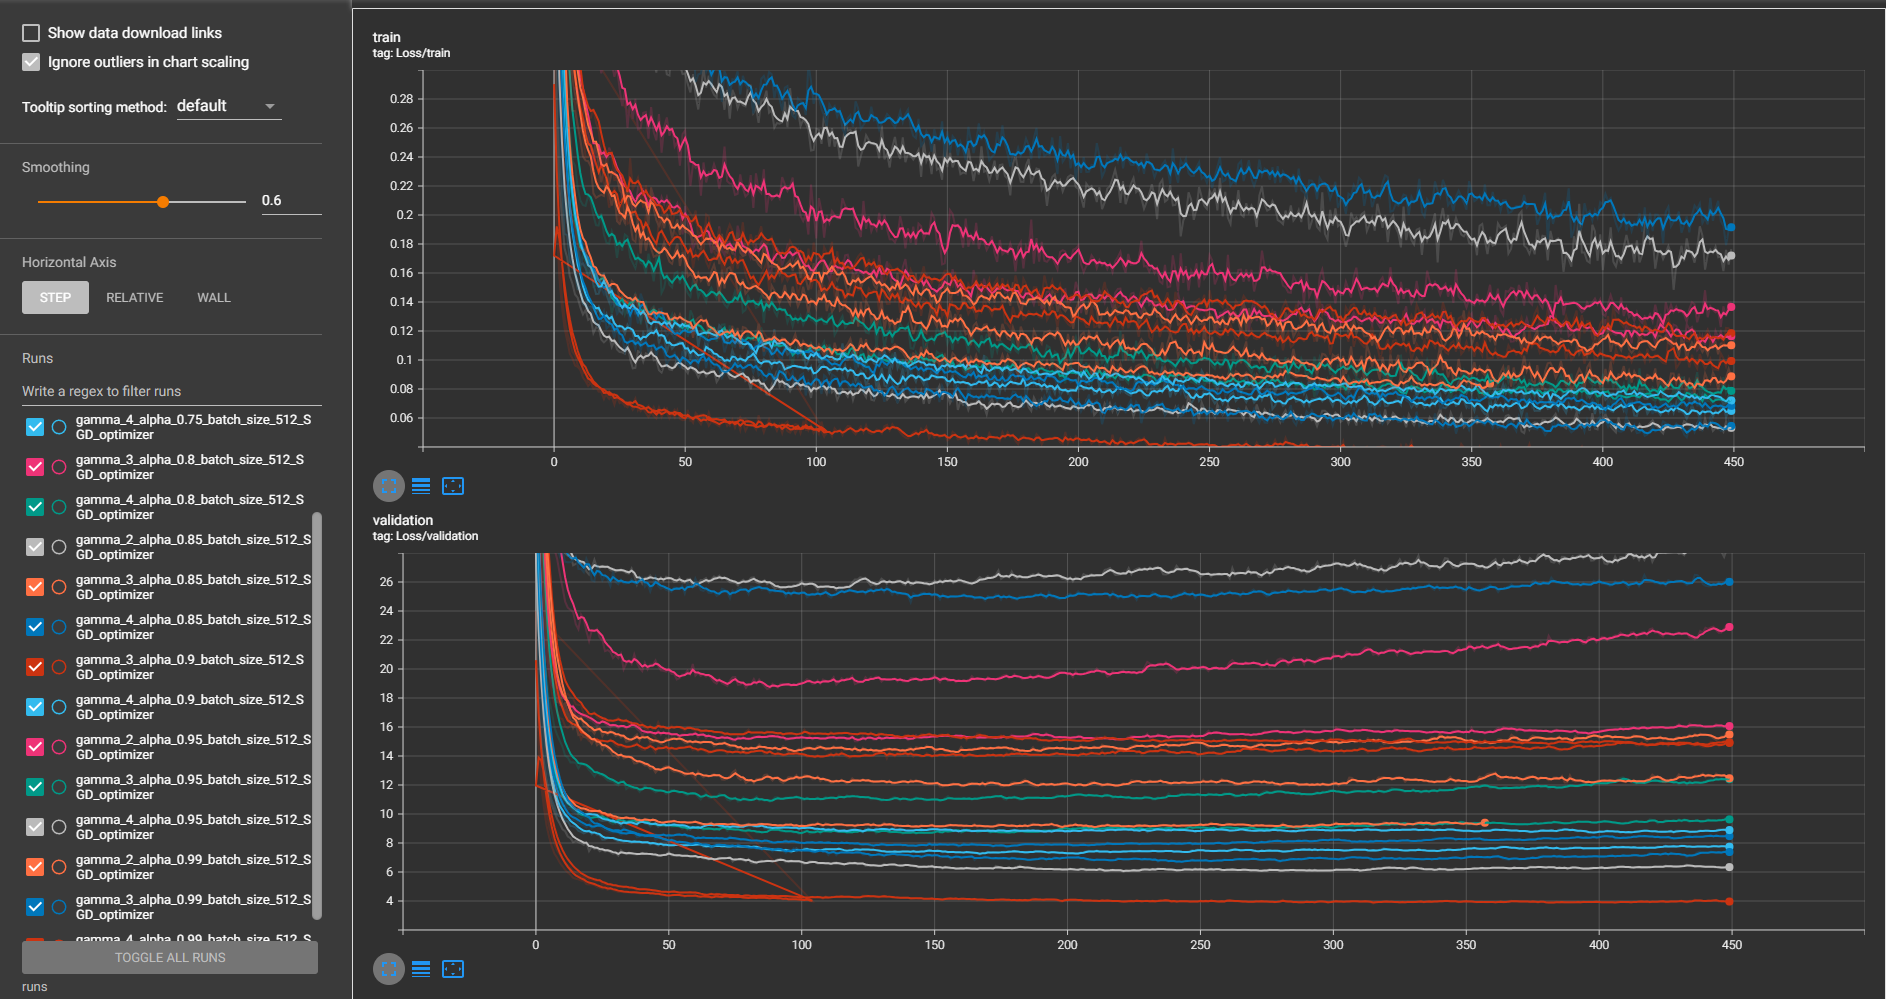
\includegraphics[width=1\linewidth]{different combination of Alpha and gamma.png}
    \caption{Different alpha and gamma effect Loss curve}
    \label{fig:Alpha and gamma}
\end{figure}

\subsection{Results}
\begin{figure}[h]
    \centering
    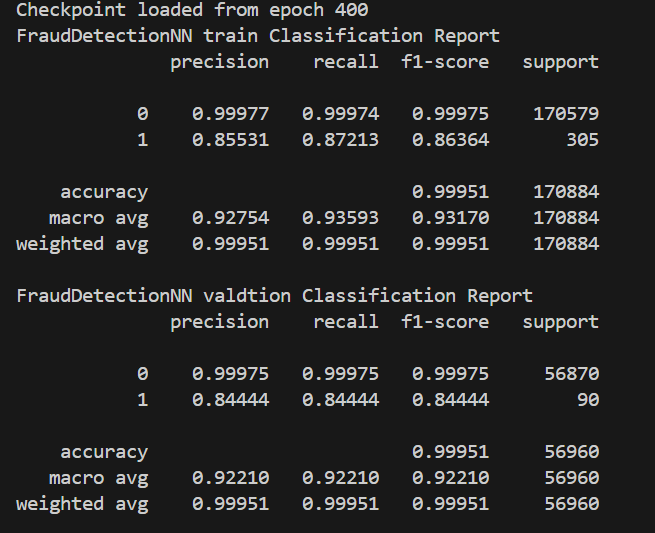
\includegraphics[width=0.8\linewidth]{Focal loss classification report.png}
    \caption{Focal loss classification report}
    \label{fig:Focal loss classification report}
\end{figure}



\newpage
\section{Smote and under-sampling technique}

SMOTE (Synthetic Minority Over-sampling Technique) is an oversampling method used to generate synthetic samples for the minority class. Despite experimenting with SMOTE, random over-sampling, and under-sampling techniques, the results on the validation data were poor.


\begin{figure}[h]
    \centering
    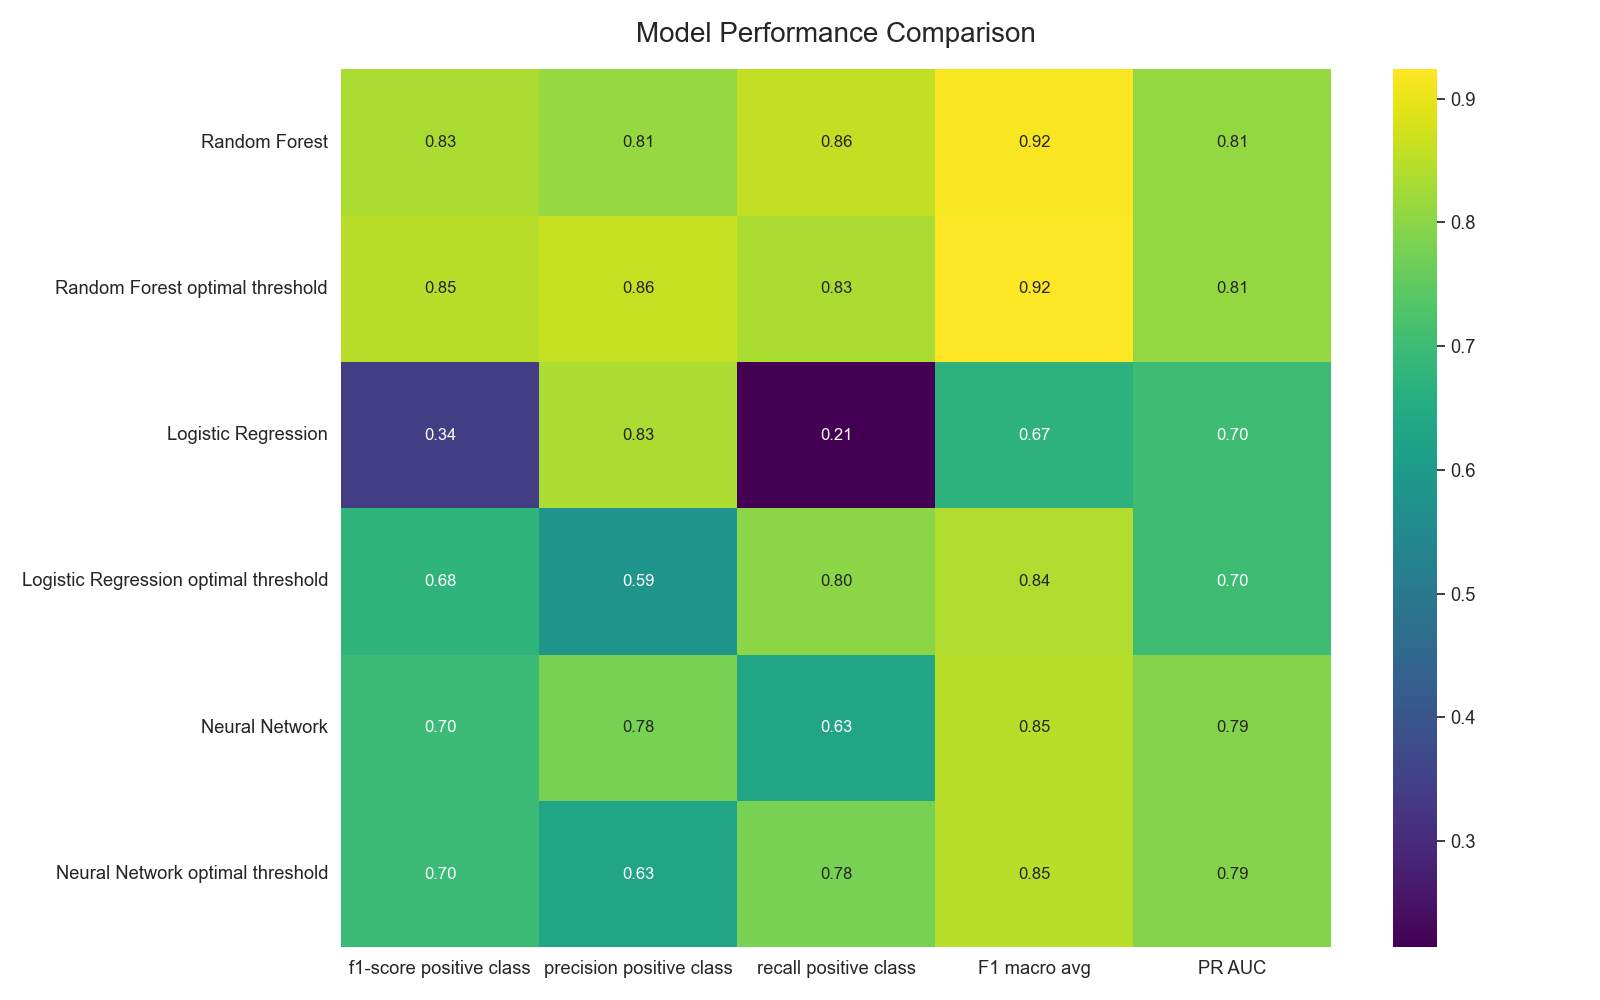
\includegraphics[width=0.80\linewidth]{Smote (0.05-ratio).png}
    \caption{Smote (0.05-ratio)}
    \label{fig:Smote (0.05-ratio)}
\end{figure}

\begin{figure}[h]
    \centering
    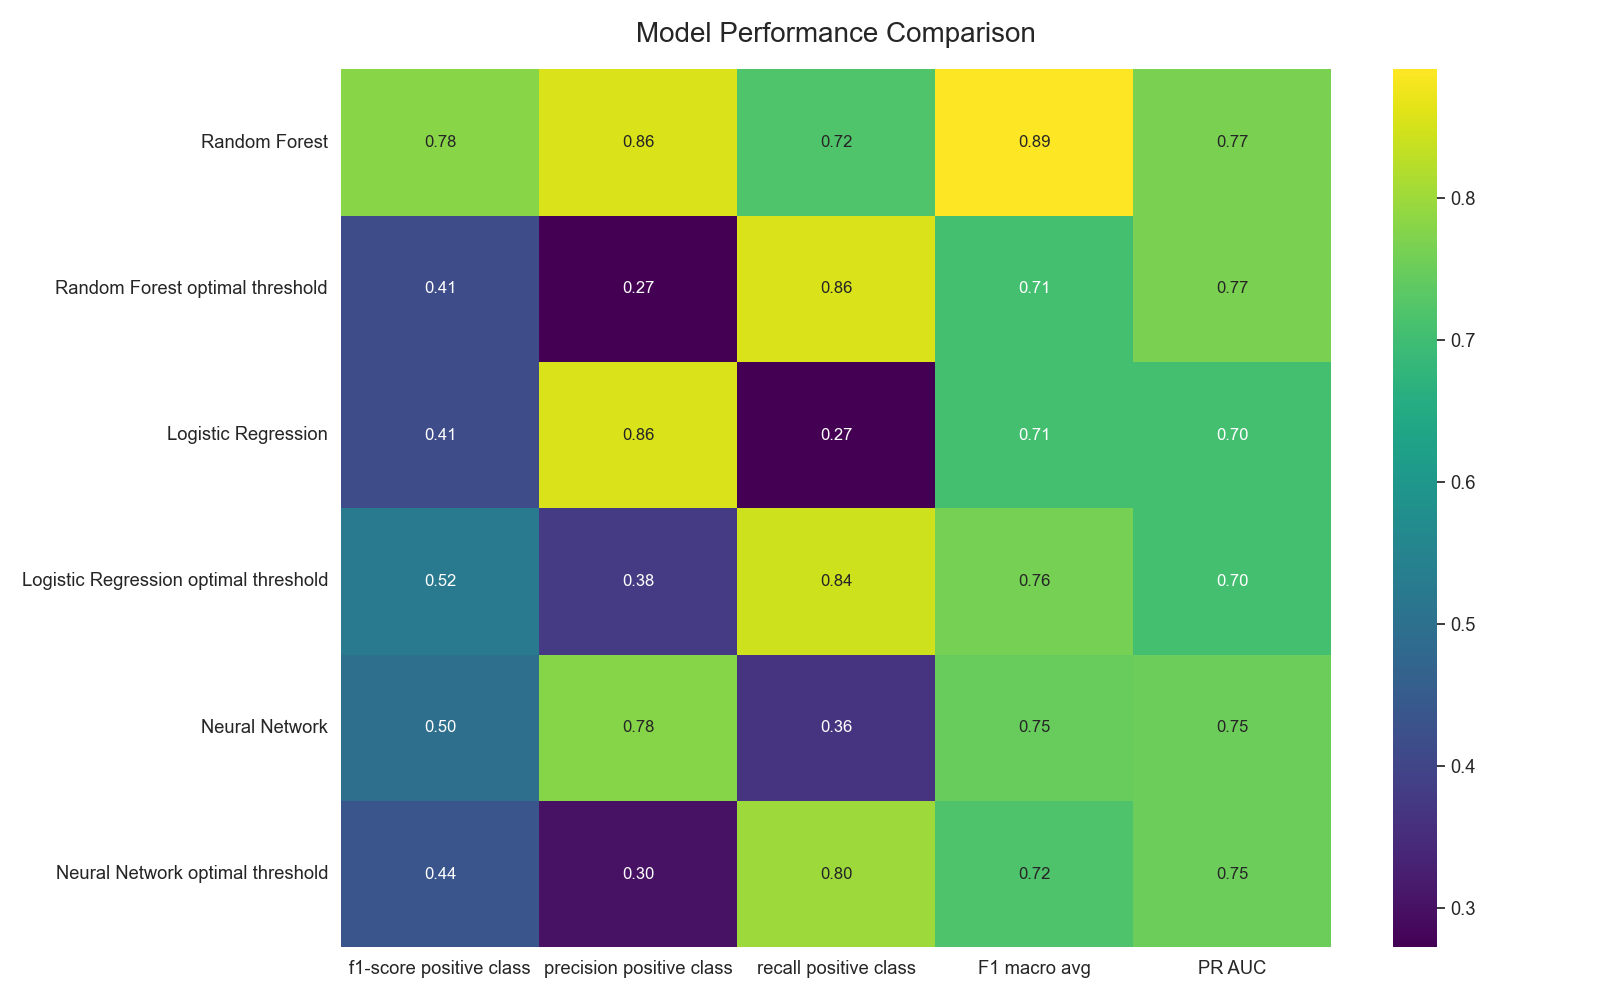
\includegraphics[width=0.80\linewidth]{RandomUnderSampler (0.05-ratio) results.png}
    \caption{Random-Under-Sampler (0.05-ratio) result}
    \label{fig:enter-label}
\end{figure}
%------------------------------------------------------------------
% Skjal endar hér
%------------------------------------------------------------------

% Heimildir
% \bibliographystyle{plain}
% \bibliography{references}
\end{document}
